\documentclass[titlepage,a4paper,12pt]{report}
\usepackage{amssymb,amsfonts,amsmath}
\usepackage{fullpage}
\usepackage{graphicx}
%\usepackage[cc]{titlepic}
\usepackage{amsthm}
\newtheorem{definition}{Definition}[section]
\newtheorem{example}{Example}[section]
\newtheorem{theorem}{Theorem}[section]
\newtheorem{exercise}{Exercise}[section]
\newtheorem{corollary}{Corollary}[section]
\newtheorem{proposition}{Proposition}[section]
\pdfpagewidth 8.5in
\pdfpageheight 11in
\setlength\topmargin{-0.5in}
\setlength\headheight{0in}
\setlength\headsep{0in}
\setlength\textheight{9.5in}
\setlength\textwidth{7.0in}
\setlength\oddsidemargin{-0.5in}
\setlength\evensidemargin{1.0in}
\setlength\parindent{0.25in}
\setlength\parskip{0.25in}
%\begin{titlepage}
%\usepackage{titlepic}
%\titlepic{
\includegraphics[width=0.2\textwidth]{uz1.png}}
%
%\title{\textbf{HMTH111 Calculus 2}}
%\author{Nhawu. G\\
%		Department of Mathematics\\
%		University of Zimbabwe, ZIM}
%
%\end{titlepage}

\begin{document}
\begin{titlepage}
 
\begin{center}
 
 
% Upper part of the page

\includegraphics[width=0.15\textwidth]{uz1.png}\\[1cm]
 
\textsc{\LARGE University of Zimbabwe}\\[1.5cm]
 
\textsc{\Large HMTHCS111 CALCULUS 2}\\[0.5cm]
 
 
% Title

{ \huge \bfseries Calculus of Several Variables}\\[0.4cm]
 

 
% Author and supervisor
\begin{minipage}{0.4\textwidth}
\begin{center} \large
\emph{Author:}\\
G. \textsc{Nhawu}
\end{center}
\end{minipage}
\begin{minipage}{0.4\textwidth}
\begin{flushright} \large
\emph{Department:} \\
\textsc{Mathematics and Computational Sciences}
\end{flushright}
\end{minipage}

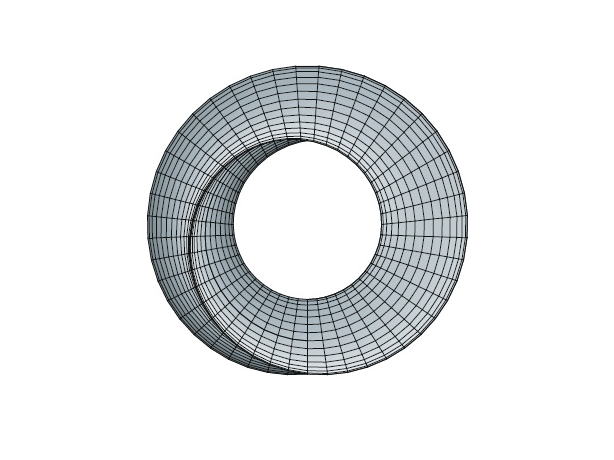
\includegraphics[width=0.7\textwidth]{umblictorus.png}\\[1cm]
 \vfill
 
 
% Bottom of the page
{\large \today}
 
\end{center}
 
\end{titlepage}
%\maketitle
\tableofcontents
\setcounter{chapter}{2}
\chapter{Lines and Planes in Space}\begin{center}
	\small{\parbox{18cm}{
		\begin{raggedright}
		{\small
		\textit{Gravity explains the motions of the planets, but it cannot explain who sets the planets in motion.}
 }
 
				\vspace{.5cm}\hfill{--- Isaac Newton}
		\end{raggedright}
	}
} 
\end{center}

In the plane, \textbf{slope} is used to determine an equation of a line. In space, it is more convenient to use \textbf{vectors} to determine the equation of a line.
\section{Vector Equation of a Straight Line}
Just as in finding the equation of a straight line in Cartesian coordinates, we will find that there are two cases to consider when finding the equation of a straight line in terms of vectors.

\noindent\textbf{Case I:}\\
One case is when you are given a fixed point on the straight line and a vector parallel to the straight line. This case is analogous to the situation in Cartesian coordinates when one is given a point through which a straight line passes and the gradient of the line is known.

\noindent Suppose the straight line $l$ passes through a point $A$ with position vector \textbf{a} with respect to our reference point $O$. Further, suppose the vector \textbf{b} is parallel to the straight line. Let $R$ be any point on the straight line and let its position vector relative to $O$ be \textbf{r}. We have \begin{eqnarray}
\overrightarrow{OR}=\overrightarrow{OA}+\overrightarrow{AR}.\nonumber
\end{eqnarray} Since $\overrightarrow{AR}$ is parallel to the vector \textbf{b}, $\overrightarrow{AR}=\lambda\textbf{b}$ where $\lambda$ is a real number. Hence the vector equation of a straight line is given by\begin{eqnarray}\label{vc1}
\textbf{r}=\textbf{a}+\lambda\textbf{b}.
\end{eqnarray}
\noindent\textbf{Case II:}\\
Suppose you are given two points through which the straight line passes.

\noindent Suppose a straight line $l$ passes through two points $A$ and $B$ with position vectors \textbf{a} and \textbf{b} respectively relative to the reference point $O$. Let $R$ be any point on the straight line and let its position vector relative to $O$ be \textbf{r}. We have \begin{eqnarray}
\overrightarrow{OR}=\overrightarrow{OA}+\overrightarrow{AR}. \nonumber
\end{eqnarray}But $\overrightarrow{AR}=\lambda\overrightarrow{AB}$ where $\overrightarrow{AB}=\textbf{b}-\textbf{a}$.\\
Thus $\textbf{r}=\textbf{a}+\lambda(\textbf{b}-\textbf{a})=(\textbf{a}-\lambda\textbf{a})+\lambda\textbf{b}=(1-\lambda)\textbf{a}+\lambda\textbf{b}$. Therefore the vector equation of a straight line in this case is given by \begin{eqnarray}\label{vc2}
\textbf{r}=(1-\lambda)\textbf{a}+\lambda\textbf{b}.
\end{eqnarray}
\section{The Cartesian Equation of a Straight Line}
We know that the general equation of a straight line in 2 dimensions has the form $ax+by+c=0$ or the equivalent form $y=mx+c$.\\
You might expect the general equation of a straight line in 3 dimensional space to have the form $ax+by+cz+d=0$. In fact this is the general equation of a \textbf{plane} and \textbf{not} a straight line. In general, there are two Cartesian coordinate forms of the equation of a straight line in 3 dimensional space namely:
\begin{enumerate}
\item parametric equations form
\item symmetric equations form.
\end{enumerate}They are all derived from the vector equation \eqref{vc1}.

\noindent\textbf{Parametric Equations}\\~\\
Suppose vectors \textbf{r}, \textbf{a}, \textbf{b} have column vectors $\begin{pmatrix}
x\\
y\\
z
\end{pmatrix}$, $\begin{pmatrix}
x_1\\
y_1\\
z_1
\end{pmatrix}$, $\begin{pmatrix}
x_2\\
y_2\\
z_2
\end{pmatrix}$ respectively and suppose \\
$\textbf{r}=\textbf{a}+\lambda\textbf{b}$ is the vector equation of straight line $l$.\\
Then $\begin{pmatrix}
x\\
y\\
z
\end{pmatrix}=\begin{pmatrix}
x_1\\
y_1\\
z_1
\end{pmatrix}+\lambda\begin{pmatrix}
x_2\\
y_2\\
z_2
\end{pmatrix}$. \\
Thus, we have \begin{eqnarray}\label{par} x=x_1+\lambda x_2,~~~y=y_1+\lambda y_2,~~~z=z_1+\lambda z_2\end{eqnarray}
These are the parametric equations of the straight line $l$ with parameter $\lambda$ in 3 dimensional space.

\noindent\textbf{Symmetric Equations}\\~\\
From the equations in \eqref{par}, we obtain \begin{eqnarray}
\frac{x-x_1}{x_2}=\frac{y-y_1}{y_2}=\frac{z-z_1}{z_2}=\lambda.\nonumber
\end{eqnarray}Hence, we have \begin{eqnarray}\label{sym}
\frac{x-x_1}{x_2}=\frac{y-y_1}{y_2}=\frac{z-z_1}{z_2}.
\end{eqnarray}These are the symmetric form of the Cartesian equations of a straight line in 3 dimensional space.

\noindent Consider the line $L$ through the point $P=(x_1,y_1,z_1)$ and parallel to vector ${\bf{A}}=(a,b,c)$. The vector ${\bf{A}}$ is the \textbf{direction vector} for the line $L$, and $a,b,c$ are the \textbf{direction numbers}. One way of describing the line $L$ is to say that it consists of all points $Q=(x,y,z)$ for which the vector $\overrightarrow{PQ}$ is parallel to ${\bf{A}}$. This means that $\overrightarrow{PQ}$ is a scalar multiple of ${\bf{A}}$, and you can write $\overrightarrow{PQ}=t{\bf{A}}$, where $t$ is a scalar.
\[\overrightarrow{PQ}=(x-x_1, y-y_1,z-z_1)=(at, bt, ct)=t{\bf{A}}.\]
\begin{figure}[h!]
\input{line.pic}
\caption{A line has directed vector ${\bf{A}}$}
\end{figure}
\section{Parametric and Symmetric Equations of a Line in Space}
By equating corresponding components, you can obtain the \textbf{parametric equations} of a line in space. 
\begin{theorem}
A line $L$ parallel to the vector ${\bf{A}}=(a,b,c)$ and passing through the point\\ $P=(x_1,y_1,z_1)$ is represented by the \textbf{parametric equations}
\[ x=x_1+at, \quad y=y_1+bt, \quad z=z_1+ct. \]
\end{theorem} 
\subsection{Symmetric Equations}
If the direction numbers $a,b,c$ are all non-zero, then you can eliminate the parameter $t$ to obtain the \textbf{symmetric equations} of a line.
\[\dfrac{x-x_1}{a}=\dfrac{y-y_1}{b}=\dfrac{z-z_1}{c}.\]
\begin{example}
Find parametric and symmetric equations of the line $L$ that passes through  the point $(1,-2,4)$ and is parallel to ${\bf{A}}=(2,4,-4)$.

\noindent \textbf{Solution:} To find a set of parametric equations of the line, use the coordinates $x_1=1, y_1=-2$ and $z_1=4$ and the direction numbers $x_2=2, y_2=4$ and $z_2=-4$.
\[x=1+2\lambda, \quad y=-2+4\lambda, \quad z=4-4\lambda.\]
Because $x_2,~y_2$ and $z_2$ are all non-zero, a set of symmetric equations is 
\[\dfrac{x-1}{2}=\dfrac{y+2}{4}=\dfrac{z-4}{-4}.\]
\end{example}
\noindent Neither the parametric equations nor the symmetric equations of a given line are unique. 
\begin{example}
Find a set of parametric equations of the line that passes through the points $(-2,1,0)$ and $(1,3,5)$. 

\noindent \textbf{Solution:} Begin by letting $P=(-2,1,0)$ and $Q=(1,3,5)$. Then a direction vector for the line passing through $P$ and $Q$ is given by 
\[{\bf{A}}=(1-(-2), 3-1, 5-0)=(3,2,5)=(x_2,y_2,z_2).\]
Using the direction numbers $x_2=3, y_2=2$ and $z_2=5$, with the point $P=(-2,1,0)$ you can obtain the parametric equations 
\[x=-2+3\lambda, \quad y=1+2\lambda, \quad z=5\lambda.\]
\end{example}
\section{Planes in Space}
We have seen how an equation of a line in space can be obtained from a point on the line and a vector \textit{parallel} to it. Now we will see that an equation of a plane in space can be obtained from a point in the plane and a vector \textit{normal} (perpendicular) to it.

\noindent Consider the plane containing the point $P=(x_1,y_1,z_1)$ and having a non-zero normal vector ${\bf{n}}=(a,b,c)$. This plane consists of all points $Q=(x,y,z)$ for which vector $\overrightarrow{PQ}$ is orthogonal to ${\bf{n}}$. Using the dot product, we have the following 
\begin{eqnarray*}
{\bf{n}\cdot}\overrightarrow{PQ} &=& 0\\
(a,b,c)\cdot (x-x_1,y-y_1,z-z_1) &=& 0\\
a(x-x_1)+b(y-y_1)+c(z-z_1) &=& 0.
\end{eqnarray*} 
The third equation of the plane is said to be in \textbf{standard form}.
\subsection{Standard Equation of a Plane in Space}
\begin{theorem}
The plane containing the point $(x_1,y_1,z_1)$ and having a normal vector ${\bf{n}}=(a,b,c)$ can be represented, in \textbf{standard form} by the equation
\[a(x-x_1)+b(y-y_1)+c(z-z_1) = 0.\]
\end{theorem}
\noindent By regrouping terms, we obtain the \textbf{general form} of the equation of a plane in space, 
\[ax+by+cz+d=0.\]
Given the general form of the equation of a plane, it is easy to find a normal vector to the plane. simply use the coefficients of $x,y$ and $z$ and write ${\bf{n}}=(a,b,c)$.
\begin{example}
Find the general equation of the plane containing the points $(2,1,1), (0,4,1)$ and $(-2,1,4)$.

\noindent \textbf{Solution:} We need a point in the plane and a vector that is normal to the plane. There are three choices for the point, but no normal vector is given. To obtain a normal vector, use the cross product of vectors ${\bf{B}}$ and ${\bf{C}}$ extending from the point $(2,1,1)$ to the points $(0,4,1)$ and $(-2, 1,4)$. The component forms of ${\bf{B}}$ and ${\bf{C}}$ are 
\begin{eqnarray*}
{\bf{B}} =(0-2, 4-1, 1-1) =(-2,3,0)\\
{\bf{C}} =(-2-2,1-1,4-1)= (-4,0,3)
\end{eqnarray*}
and it follows that 
\[{\bf{n}=\bf{B}\times \bf{C}}=\begin{vmatrix}
{\bf{i}} & {\bf{j}} & {\bf{k}}\\
-2 & 3 & 0 \\
-4 & 0 & 3
\end{vmatrix}=9{\bf{i}}+6{\bf{j}}+12{\bf{k}}=(a,b,c)\] is normal to the given plane. Using the direction numbers for ${\bf{n}}$ and the point $(x_1,y_1,z_1)=(2,1,1)$, you can determine an equation of the plane to be 
\begin{eqnarray*}
a(x-x_1)+b(y-y_1)+c(z-z_1) &=& 0 \\
9(x-2)+6(y-1)+12(z-1) &=& 0 \quad (Standard\, form)\\
9x+6y+12z-36 &=& 0\\
3x+2y+4z-12 &=& 0. \quad (General\, form)
\end{eqnarray*}
\textbf{Remark:} Check to see that each of the three points satisfies the equation $3x+2y+4z-12=0$.
\end{example}
\section{Angle Between Two Planes}
Two distinct planes in three-dimensional space either are parallel or intersect in a line. If they intersect, you can determine the angle between them from the angle between their normal vectors. Specifically, if vectors ${\bf{n}}_1$ and ${\bf{n}}_2$ are normal to two intersecting planes, the the angle $\theta $ between the normal vectors is equal to the angle between the two planes and is given by 
\[\cos \theta =\dfrac{{\bf{n}}_1 \cdot {\bf{n}}_2}{|{\bf{n}}_1||{\bf{n}}_2|}.\]
Consequently, two planes with normal vectors ${\bf{n}}_1$ and ${\bf{n}}_2$ are 
\begin{enumerate}
\item \textit{perpendicular}, if ${\bf{n}}_1\cdot {\bf{n}}_2 =0$.
\item \textit{parallel}, if ${\bf{n}}_1$ is a scalar multiple of ${\bf{n}}_2$.
\end{enumerate}
\begin{example}
Find the angle between the two planes
\begin{eqnarray*}
x-2y+z &=& 0 \quad Equation\, for\, Plane\, 1\\
2x+3y-2z &=& 0 \quad Equation\, for\, Plane\, 2
\end{eqnarray*} 
and find parametric equations of their line of intersection. 
\end{example}

\noindent \textbf{Solution:} The normal vectors for the planes are ${\bf{n}}_1=(1,-2,1)$ and ${\bf{n}}_2=(2,3,-2)$. Consequently, the angle between the two planes is as follows 
\begin{eqnarray*}
\cos \theta &=& \dfrac{{\bf{n}}_1 \cdot {\bf{n}}_2}{|{\bf{n}}_1||{\bf{n}}_2|} \\
&=& \dfrac{-6}{\sqrt{6}\sqrt{17}} \\
&=& \dfrac{-6}{\sqrt{102}} \\
&\approx & -0.59409 \quad (\theta \approx \cos ^{-1} -0.59409).
\end{eqnarray*} 

\noindent You can find the line of intersection of the two planes by simultaneously solving the two linear equations representing the planes. Multiply the first equation by $-2$ and add the result to the second equation.
\begin{eqnarray*}
-2x +4y-2z = 0\\
\underline{2x+3y-2z = 0} \\
0x +7y-4z=0.
\end{eqnarray*}
So $y=\dfrac{4z}{7}$. Substituting this into one of the original equations, we have $x=\dfrac{z}{7}$. Finally, letting $t=\dfrac{z}{7}$, we obtain the parametric equations 
\[x=t, \quad y=4t, \quad z=7t \quad (\mbox{Line of Intersection} ).\]  

\section{Distances Between Points, Planes and Lines}
In this section we want to find two basic types of distance problems in space, 
\begin{enumerate}
\item Finding the distance between a point and a plane.
\item Finding the distance between a point and a line.
\end{enumerate}
The solutions of these problems illustrate the versatility and usefulness of vectors in coordinate geometry. The first problem uses the \textit{dot product} of two vectors, and the second problem uses the \textit{cross product}.  The distance $D$ between a point $Q$ and a plane is the length of the shortest line segment connecting $Q$ to the plane. 
\subsection{Distance Between a Point and a Plane}
\begin{theorem}
The distance between a plane and a point $Q$ (not in the plane) is 
\[D=\dfrac{|\overrightarrow{PQ}\cdot {\bf{n}}|}{|{\bf{n}}|}.\]
\end{theorem}
To find a point in the plane given by $ax+by+cz+d=0 \, (a\neq 0)$, let $y=0$ and $z=0$. Then, from the equation $ax+d=0$, we conclude that the point $(-\frac{d}{a}, 0, 0)$ lies in the plane.
\begin{example}
Find the distance between $Q=(1,5,-4)$ and the plane given by $3x-y+2z=6$.

\noindent \textbf{Solution:} We know that ${\bf{n}}=(3,-1,2)$ is normal to the given plane. To find a point in the plane, let $y=0$ and $z=0$, and obtain the point $P=(2,0,0)$. The vector from $P$ to $Q$ is given by 
\[\overrightarrow{PQ}=(1-2, 5-0, -4-0)=(-1, 5, -4).\]
Using the distance formula, 
\begin{eqnarray*}
D=\dfrac{|\overrightarrow{PQ}\cdot {\bf{n}}|}{|{\bf{n}}|} &=& \dfrac{|(-1,5,-4)\cdot (3,-1,2)|}{\sqrt{9+1+4}} \\
&=& \dfrac{|-3-5-8|}{\sqrt{14}}\\
&=& \dfrac{16}{\sqrt{14}}.
\end{eqnarray*}
\textbf{Remark:} The choice of the point $P$ is arbitrary in the Example. Try choosing a different point to verify that we obtain the same distance.
\end{example}
The distance between the point $Q=(x_0, y_0, z_0)$ and the plane given by $ax+by+cz+d=0$ is 
\begin{eqnarray*}
D &=& \dfrac{|a(x_0-x_1)+b(y_0-y_1)+c(z_0-z_1)|}{\sqrt{a^2+b^2+c^2}}\\
D &=& \dfrac{|ax_0+by_0+cz_0+d|}{\sqrt{a^2+b^2+c^2}}
\end{eqnarray*}
where $P=(x_1,y_1,z_1)$ is a point on the plane and $d=-(ax_1+by_1+cz_1)$.
\section{Finding the Distance Between Two Parallel Planes}
\begin{example}
Find the distance between the two parallel planes given by $3x-y+2z-6=0$ and $6x-2y+4z+4=0$.

\noindent \textbf{Solution:} To find the distance between the planes, choose a point in the first plane, say $(x_0,y_0,z_0)=(2,0,0)$. Then, from the second plane, we determine that $a=6, b=-2, c=4$ and $d=4$, and conclude that the distance is 
\begin{eqnarray*}
D &=& \dfrac{|ax_0+by_0+cz_0+d|}{\sqrt{a^2+b^2+c^2}} \\
&=& \dfrac{|6(2)+(-2)(0)+(4)(0)+4|}{\sqrt{6^2+(-2)^2+4^2}}\\
&=& \dfrac{16}{\sqrt{56}} =\dfrac{8}{\sqrt{14}} \approx 2.14.
\end{eqnarray*}
\end{example}
\section{Distance Between a Point and a Line in Space }
The formula for the distance between a point and a line in space resembles that for the distance between a point and a plane, except that we replace the dot product by the cross product and replace the normal vector ${\bf{n}}$ by a direction vector for the given line. 
\begin{theorem}
The distance between a point $Q$ and a line in space is given by 
\[D=\dfrac{|\overrightarrow{PQ}\times {\bf{u}}|}{|{\bf{u}}|}\] where ${\bf{u}}$ is the direction vector for the line and $P$ is a point on the line.
\end{theorem}
\begin{example}
Find the distance between the point $Q=(3,-1,4)$ and the line given by 
\[x=-2+3t, \quad y=-2t, \quad z=1+4t.\]

\noindent \textbf{Solution:} Using the direction numbers, $3, -2$ and $4$, we know that the direction vector for the line is ${\bf{u}}=(3,-2,4)$. To find a point on the line, let $t=0$, and obtain $P=(-2,0,1)$. thus, 
\[\overrightarrow{PQ}=(3-(-2), -1-0,4-1)=(5,-1,3)\] and we form the cross product 
\[\overrightarrow{PQ} \times {\bf{u}} =\begin{vmatrix}
{\bf{i}} & {\bf{j}} & {\bf{k}} \\
5 & -1 & 3 \\
3 & -2 & 4
\end{vmatrix}=2{\bf{i}}-11{\bf{j}}-7{\bf{k}}=(2,-11,-7).\] Finally 
\[D=\dfrac{|\overrightarrow{PQ}\times {\bf{u}}|}{|{\bf{u}}|} =\dfrac{\sqrt{174}}{\sqrt{29}} =\sqrt{6}\approx 2.45.\]
\end{example}

\section{Tutorial Questions}
\begin{enumerate}
\item Find the parametric and symmetric equations of the line through the two points.\\
(i)\,  $(5,-3,-2)$ and $(-\frac{2}{3}, \frac{2}{3},1)$ \quad (ii)\, $(1,0,1)$ and $(1,3,-2)$.
\item Determine which of the points lie on the line $L$.
\begin{itemize}
\item[(a)] The line $L$ passes through the point $(-2,3,1)$ and is parallel to the vector ${\bf{A}}=4{\bf{i}}-{\bf{k}}$.  \\
(i)\, $(2,3,0)$ \quad (ii)\, $(-6,3,2)$ \quad (iii)\, $(2,1,0)$ \quad (iv)\, $(6,3,-2)$.
\item[(b)] The line $L$ passes through the points $(2,0,-3)$ and $(4,2,-2)$.\\
(i)\, $(4,1,-2)$ \quad (ii)\, $(\frac{5}{2}, \frac{1}{2}, -\frac{11}{4})$ \quad (iii)\, $(-1, -3, -4)$ \quad $(0,-2,-4)$.
\end{itemize}
\item Find the parametric equation of the line that passes through the point $(2,3,4)$ and is perpendicular to the plane given by $3x+2y-z=6$.
\item Find the equation of the plane that contains the point $(1,-2,3)$ and is parallel to the plane $z=2x+3y-4$.
\item Find the equation of the plane passing through the points\\
(i)\, $(0,0,0), (1,2,3)$ and $(-2,3,3)$ \quad (ii)\, $(1,2,-3), (2,3,1)$ and $(0,-2,-1)$ \\
(iii)\, $(1,2,3), (3,2,1)$ and $(-1,-2,2)$.
\item Determine whether the planes are parallel or orthogonal or neither. If they are neither parallel nor orthogonal, find the angle between them.\\
(i)\, $5x-3y+z=4,\,  x+4y+7z=1$ \quad (ii)\, $3x+y-4z=3, \, -9x-3y+12z=4$\\
(iii)\, $x-3y+6z=4, \, 5x+y-z=4$ \quad (iv)\, $3x+2y-z=7, \, x-4y+2z=0$\\
(v)\, $x-5y-z=1, \, 5x-25y-5z=-3 $ \quad (vi)\, $2x-z=1, \, 4x+y+8z=10$.
\item Find the angle of intersection of the plane $x+y-z=0$ and the plane $x-3y+z-1=0$.
\item Given the planes $3x+y-5=0, \, y+z-1=0$. Determine equations of the line of intersection of the planes.
\item Find the parametric equations for the line of intersection of the planes.\\
(i)\, $3x+2y-z=7, \, x-4y+2z=0$ \quad (ii)\, $x-3y+6z=4, \, 5x+y-z=4$ \quad (iii)\, $2x+y+z=4, \,3x-y+z=3$.
\item Find the parametric equations of the line of intersection of the planes $2x+y+z=4$ and $3x-y+z=3$.
\item Find the distance between the point $(10,3,-2)$ and the line $x=4t-2, \, y=3, \, z=-t+1$.
\item Find the distance between the point $(4,1,-2)$ and the line $x=2t+2, \, y=2t, \, z=t-3$.
\item Find the distance between the point $(0,0,0)$ and the plane $2x+3y+z=12$.
\item Find the distance from the point $(2,5,4)$ to the plane $x+2y+2z=2$.
\item Find the distance between the point $(1,2,3)$ and the plane $2x-y+z=4$.
\item Find the distance between the planes.\\
(i)\, $x-3y+4z=10, \, x-3y+4z=6$ \quad (ii)\, $2x-4z=4, \, 2x-4z=10$\\
(iii)\, $2x-3y+z=6, \, 2x-3y+z=2$ \quad (iv)\, $x+2y-z=0, \, x+2y-z=4$.
\item A plane passes through the point $(1,1,1)$ and is perpendicular to each of the planes $3x-2y+3z+6=0$ and $6x-2y-3z-6=0$. Find its equation.
\item Given three points $(1,2,3), \, (-1,3,1)$ and $(-2,-3,0)$, find the equation of the plane through these points.
\item Find an equation for the plane that passes through the point $(1,3,-2)$ and also passes through the line of intersection of the planes $x-y+z=1$ and $x+y-z=1$.
\item Find the equation of the plane through the points $(1,0,-1)$ and $(2,1,0)$ that is also parallel to the line of intersection of the planes $x+y+z=5$ and $3x-y=4$.
\end{enumerate}
\end{document}